\documentclass[11pt]{article} % 
\usepackage[pdftex]{graphicx}
\usepackage{fullpage}
\usepackage{graphicx}
\usepackage{graphics}
\usepackage{psfrag}
\usepackage{pgf}
\usepackage{color}
\usepackage{tikz}
\usetikzlibrary{arrows,automata}
\usepackage[latin1]{inputenc}
\usepackage{amsthm}
\usepackage{amsmath,amssymb}
\usepackage{enumerate}
\setlength{\textwidth}{6.5in}
\setlength{\textheight}{9in}
\newcommand{\N}{\mathbb{N}}
\newcommand{\Z}{\mathbb{Z}}
\newcommand{\R}{\mathbb{R}}
\newcommand{\Q}{\mathbb{Q}}
\newcommand{\C}{\mathbb{C}}
\newcommand{\PP}{\mathbb{P}}
\newcommand{\tab}{\;\;\;\;\;}
\newcommand{\inv}{^{-1}}
\newcommand{\tr}{\textrm}
\newcommand{\lc}{\sqcup}
\newcommand{\var}{\tr{Var}}
\newcommand{\cov}{\tr{Cov}}
\newcommand{\like}{\mathcal{L}}

\begin{document}

\hfill Robert Johns

\hfill March 13, 2014

\begin{center} {\Large CSCI 678: Statistical Analysis of Simulation Models}\\{\large Homework 7}\end{center}

\begin{enumerate}

%%%%%
%1
\item

\begin{enumerate}

%1a
\item $$F(x) = \left\{\begin{array}{ll}\frac{(x - a)^2}{(b-a)(c-a)} & a \le x < c \\ 1-\frac{(b-x)^2}{(b-a)(b-c)} & c \le x < b\\ 1 & x \ge b \end{array}\right.$$

%1b
\item $$F\inv(u) = \left\{\begin{array}{ll} a + \sqrt{u(b-a)(c - a)} & 0 \le u < (c-a)/(b-a) \\ b - \sqrt{(1 - u)(b-a)(b - c)} & (c-a)/(b-a) \le u \le 1\end{array}\right.$$

%1c
\item The program \texttt{asm7a.c} contains the function and the handwritten analytic work, and is attached at the end.  Variates, along with the mean are printed on a separate sheet.

%1d
\item The program \texttt{asm7a.c} contains the function and the handwritten analytic work, and is attached at the end.  Variates, along with the mean are printed on a separate sheet.

%1e
\item The program \texttt{asm7a.c} contains the function and the handwritten analytic work, and is attached at the end.  Variates, along with the means, are printed on a separate sheet.

%1f
\item Written on the source code is a count of computations for each algorithm.

\end{enumerate}

%%%%%
%2
\item

\begin{enumerate}

%2a
\item 

$ $

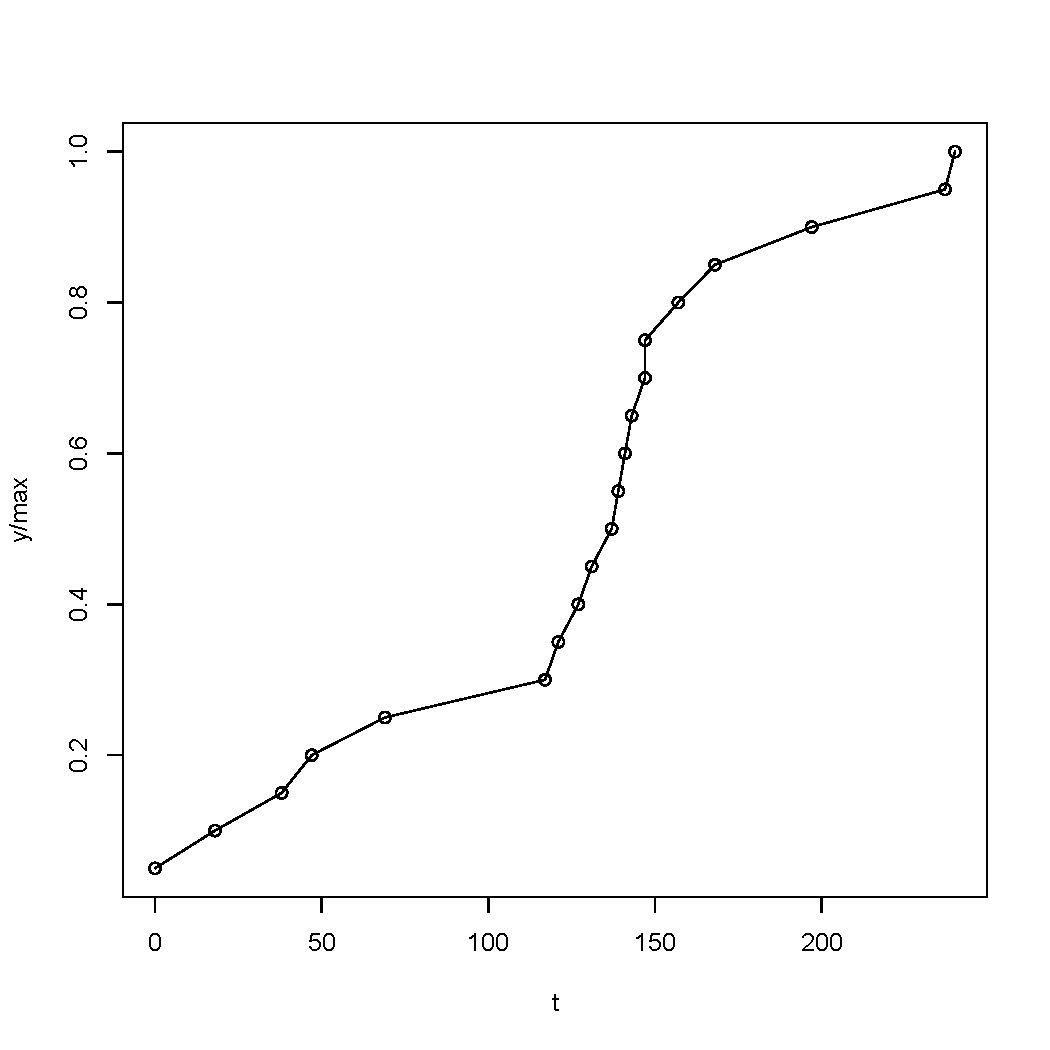
\includegraphics[scale = 0.5]{plot1.pdf}

%2b
\item The realization of the simulation yields the following variates:

\begin{verbatim}0.672, 0.344, 0.016, 5.607, 11.508, 17.410, 23.902, 30.459, 37.016, 40.508, 
43.459, 46.410, 52.770, 59.984, 67.197, 80.803, 96.541, 112.279, 117.918, 
119.230, 120.541, 122.279, 124.246, 126.213, 127.787, 129.098, 130.410, 132.082, 
134.049,136.016, 137.328, 137.984, 138.639, 139.295, 139.951, 140.607, 141.262,
141.918, 142.574, 143.459, 144.770, 146.082, 147.000, 147.000, 147.000, 147.820,
151.098, 154.377, 157.721, 161.328, 164.934, 169.426, 178.934, 188.443, 198.311,
211.426, 224.541, 237.049, 238.033, 239.016\end{verbatim}

Visual representation of how the variates were obtained is found on the above diagram in (a).

\end{enumerate}

%%%%%
%3
\item Let $Y = \min\{u_1, u_2,\ldots,u_n\}$. We see that
\begin{align*}
F_Y(y) &= P(Y\leq y)\\
&= P(\min\{u_1,\ldots u_n\} \leq y)\\
&= 1 - P(\min\{u_1, u_2, \ldots u_n\} > y)\\
&= 1 - P(u_1 > y, u_2 > y, \ldots u_n > y)\\
&= 1 - P(u_1 > y)*P(u_2 > y)*\cdots*P(u_n > y)\\
&= 1 - (1 - P(u_1 \le y))*(1 - P(u_2 \le y))*\cdots*(1 - P(u_n \le y))\\
&= 1 - (1 - F(u_1))*(1 - F(u_2))*\cdots*(1-F(u_n))\\
&= 1 - (1-F(u))^n\end{align*}
Taking the inverse, we get $Y = F\inv(u) = 1 - (1 - u)^{1/n}$

%%%%%
%4
\item As the acceptance-rejection method is a trial-until-first-success process, it's logical that we should use a geometric (I don't remember which parameterization is capitalized, but I'm talking about the distribution of the trial number of the first success) distribution.  The parameter $p = f(x) / f^*(x)$, where $f^*$ is the majorizing function and $f$ is the pdf will be $p$ in our geometric distribution.

%%%%%
%5
\item If we take $T$ to be nonnegative, then the inverse-chf method gives us that $T = H\inv(-\ln(1 - U))$.  From this, we see that $H(T) = -\ln(1 - U)$.  Applying a probability integral transformation, we can express $U$ as $F_X(X)$, where $F_X$ is the cdf for an exponential(1) random variable.  We see then that $H(T) = -\ln(1 - F_X(X)) = -\ln(e^{-X}) = X$, which we know is exponential(1).

%%%%%
%6
\item The program \texttt{asm7e.r} was used to obtain the following results:

\begin{verbatim}"Estimate:"
8.165347
"Exact Result:"
8.144789\end{verbatim}

\end{enumerate}

\end{document}